\chapter[Practical Hybrid Quantum-Classical Computing]{Practical Hybrid Quantum-Classical\\Computing} \label{chap:practical-hybrid-quantum-classical-computing}
This chapter is focused on the practical execution of \glspl{hqca} using the Quantum Inspire quantum computing platform and SURF's \gls{hpc} center.
It will start with describing the relevant platforms, followed by reviewing and analyzing how these platforms are used to execute \glspl{hqca} in different workflows.

\section{Quantum Inspire}
Quantum Inspire is a full-stack quantum computing platform that QuTech launched last year to make quantum systems available to the general public for exploratory research~\cite{last2020quantum}.
Users can run quantum circuits on different back-ends through the Quantum Inspire web editor or by using the Python \gls{sdk}.
The \gls{cqasm}~\cite{khammassi2018cqasm} is used for describing quantum circuits, but the popular quantum computing frameworks ProjectQ~\cite{steiger2018projectq} and Qiskit~\cite{qiskit} are also supported by the Python \gls{sdk}.
Quantum Inspire supports the execution of quantum circuits on real \glspl{qpu} and through quantum simulation.
An overview of the Quantum Inspire workflow and available device back-ends is shown in \Cref{fig:qi-workflow}.

The two available \glspl{qpu} are Starmon-5 and Spin-2 which have five and two qubits respectively.
These \glspl{qpu} suffer from noise, limited coherence time, limited qubit connectivity, and each \gls{qpu} has a specific allowed gate set.
Note that these gate sets are universal, and non-native gates are decomposed into supported gates depending on the \gls{qpu}.
Regardless of the limitations of these \glspl{qpu}, they are an essential part in research towards better quantum hardware and quantum algorithms.
\begin{figure}[ht]
    \centering
    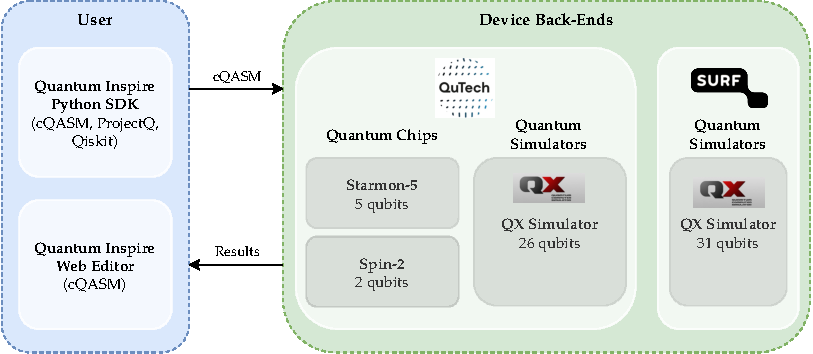
\includegraphics[width=1\linewidth]{figures/qi-workflow.pdf}
    \caption[Overview of the Quantum Inspire workflow.]{
        Overview of the Quantum Inspire workflow.
        Users can submit quantum circuits written in \gls{cqasm} using the web editor or Python \gls{sdk}.
        After the program has been run, the results are returned to the user.
        The quantum circuit can be executed on one of the \glspl{qpu} or simulated using one of the QX simulator back-ends.
        QuTech's simulator back-end supports simulations up to 26 qubits, while SURF's simulator back-end supports simulations up to 31 qubits.
    }
    \label{fig:qi-workflow}
\end{figure}

In the absence of large-scale and fault-tolerant quantum computers, quantum computer simulation is critical for developing and testing quantum algorithms.
Quantum computer simulators often use one of three classical algorithms to simulate quantum circuits.
These algorithms have different trade-offs in the resources that they use.
First, there is the naive Schr{\"o}dinger simulation algorithm in which the complex amplitudes of a quantum state are represented in a state-vector, gates are represented as matrices, and state evolution is done by matrix-vector multiplication.
This algorithm uses $O(2^n)$ time and space, where $n$ is the amount of qubits~\cite{aaronson2016complexity}.
Second, there is the Feynman simulation algorithm which makes use of the path integral formulation of quantum mechanics~\cite{feynman2005space}.
This approach uses $O(m+n)$ space, but takes $O(4^m)$ time, where $m$ is the amount of gates~\cite{aaronson2016complexity}.
So while using a linear amount of space, the time it takes grows exponential with the number of gates.
The number of gates even for small computations can reach the order of thousands.
Supercomputers may be able to simulate quantum circuits with a thousand gates using the Schr{\"o}dinger  algorithm, but not even the most powerful supercomputer could simulate such circuit using the Feynman algorithm.
On the other hand, the Feynman algorithm can simulate a quantum circuit with a few gates and 100 qubits, while the Schr{\"o}dinger algorithm is greatly limited in the amount of qubits it can simulate due to its exponential space requirement.
Finally, \textcite{aaronson2016complexity} described an algorithm that offers best of both worlds: the Schr{\"o}dinger-Feynman algorithm.
This algorithm uses $O(d^n)$ time and $O(d \cdot n \log n)$ space, where $d$ is the depth of the circuit.
These different simulation algorithms allow you to trade time for space efficiency and vice versa, but all of them require exponential time and/or space, greatly limiting the size of simulations we can do.

Quantum Inspire offers two simulator back-ends which use QX~\cite{khammassi2017qx} as quantum computer simulator.
The QX simulator uses the Schr{\"o}dinger simulation algorithm focused on efficiently using sparse operators.
One of the simulator back-ends is hosted by QuTech on a commodity cloud-based server with 4 GB of memory, which can run simulations up to 26 qubits.
The other simulator back-end is hosted on SURF's computer cluster Lisa which consists of several hundreds of multi-core nodes.
The largest node available on Lisa has 256 GB of memory, which supports simulations up to 31 qubits.

When quantum circuits are submitted to Quantum Inspire, they are handed to a job scheduler which will attempt to schedule the job as quickly as possible when the requested resources are available.
For the \glspl{qpu} and QuTech simulator back-ends, the jobs are simply placed in a queue which are executed in first-in-first-out order.
The wait time for these back-ends ranges from seconds to minutes.
For the SURF simulator back-end, the jobs are handled by a batch system.
Because SURF's infrastructure is shared with many other users, wait times can vary from minutes to hours.
Especially large simulations which require a large amount of resources may take a long time to schedule.

\section{SURF High Performance Computing}
SURF offers an integrated ICT research infrastructure and provides services in the areas of computing, data storage, visualization, networking, and cloud.
This report is mainly interested in the computing services, and more precisely the Lisa and Cartesius cluster computers.
These cluster computers can be thought of as a network of computers (nodes).
Each node has its own \glspl{cpu}, memory, disk space, and a shared file system.
Cluster computers are often used for \acrfull{hpc}, where a large amount of resources (\glspl{cpu}, \glspl{gpu}, memory etc.) are used to solve computationally expensive problems.
Interacting with a cluster computer works different than a regular computer: instead of submitting a script or command (job) and immediately being run, cluster computers use a batch system that runs your job as soon as sufficient resources are available.
Lisa and Cartesius use the Slurm workload manager~\cite{yoo2003slurm} as job scheduler.
The specifications of the Lisa and Cartesius cluster computers are described in \Cref{table:surf-cluster-computers}.
\begin{table}[ht]
    \centering
    \begin{tabular}{ c|c|c }
        Resource & Lisa & Cartesius \\
        \hline
        \glspl{cpu} & 5304 & 47,776   \\
        Memory & 41.7 TB & 130 TB \\
        \glspl{gpu} & 216 & 132 \\
        Flop/s (64-bit floating point) & 367.9 Tflop/s & 1.843 Pflop/s  \\
        Disk space & 400 TB home & 180 TB home, 7.7 PB project + scratch \\
    \end{tabular}
    \caption[Specification of the Lisa and Cartesius cluster computers.]{
        Specification of the Lisa and Cartesius cluster computers.
        Here Flop/s refers to floating point operations per second, or the theoretical peak performance.
        Cartesius is the Dutch national supercomputer meant for large computations that require many cores, large symmetric multiprocessing nodes, large amounts of memory, a fast interconnect, large amount of disk space, or a fast I/O subsystem.
        Lisa is meant for tasks that need large computing capacities, but do not need the facilities of a real supercomputer.
    }
    \label{table:surf-cluster-computers}
\end{table}

The Lisa and Cartesius cluster computers consist of login nodes and batch nodes.
One connects to the system through the login node, which is an interactive system similar to a personal computer.
These login nodes can be used for light tasks such as writing and compiling software, writing job scripts, and preparing data.
A job script is essentially a recipe of commands that you want your job job to execute.
Through this script you can load the required modules, handle input and output data processing, define the amount of resources your job requires, and handle the running of the actual application.
The job script is submitted to the job scheduler and will be run on a batch node as soon as the requested resources are available.

\section{Hybrid Quantum-Classical Workflows}
When researching and running \glspl{hqca}, different problems require different workflows.
For example, small simulation experiments do not require \gls{hpc} facilities, unless one wants to run the experiment many times in parallel with varying parameters.
In \Cref{table:hqca-workflows} the five different workflows which are considered in this report are described.
The order in which the workflows are displayed can be thought of as progressing from small experimentation and prototyping to (large) well-defined experiments.
First, the Local-Local hybrid quantum-classical workflow is often enough for most use cases as most research towards \glspl{hqca} does not require \gls{hpc} facilities or access to a \gls{qpu}.
The Local-\gls{hpc} workflow is useful for large quantum circuit simulations that exceed the resources of modern laptops.
In such case the \gls{hpc}-\gls{hpc} workflow may also be used to reduce network overhead and repeated scheduler wait times.
Generally, one wants the quantum and classical part to be as close to each other as possible, and ideally on the same network.
This is usually possible for quantum simulators, but becomes more difficult when dealing with \glspl{qpu}.
The Local-\gls{qpu} workflow is useful for experimenting and testing out quantum hardware.
In the context of \glspl{hqca}, this can be useful for running small experiments and seeing how noise affects the performance of the algorithm.
For larger and more well-defined experiments, the \gls{hpc}-\gls{qpu} workflow offers the advantage of being able to run experiments unattended.
One could for example define multiple experiments with different parameters and run it over night on SURF's cluster computer.
This is also the biggest advantage of the \gls{hpc}-\gls{hpc} workflow --- one could run many experiments in parallel instead of being limited to local resources.

\begin{table}[ht]
    \centering
    {\renewcommand{\arraystretch}{1.35}
        \begin{tabular}{ c|c|c|>{\centering\arraybackslash}m{4.9cm} }
            Workflow name & Classical part & Quantum part & Use case(s) \\
            \hline
            Local-Local & Local & Simulation (Local) & Small experimentation/prototyping \\
            \hline
            Local-\gls{hpc} & Local & Simulation (\gls{hpc}) & Large quantum simulations that can not be run locally \\
            \hline
            Local-\gls{qpu} & Local & \gls{qpu} & Small experimentation/exploration of hardware \\
            \hline
            \gls{hpc}-\gls{qpu} & \gls{hpc} & \gls{qpu} & Well-defined/multiple experiments, hybrid computation with expensive classical part \\
            \hline
            \gls{hpc}-\gls{hpc} & \gls{hpc} & Simulation (\gls{hpc}) & Multiple experiments, expensive classical and/or quantum part, high performance simulations \\
        \end{tabular}
    }
    \caption[Relevant hybrid quantum-classical workflows and their use cases.]{
        Relevant hybrid quantum-classical workflows and their use cases.
        In the classical part column the platform on which the classical computation runs: locally on a laptop or personal computer, or on SURF's \gls{hpc} center.
        Equivalently, the quantum part columns refers to the platform the quantum computation runs on: local simulation, \gls{qpu}, or simulation on SURF's \gls{hpc} center.
    }
    \label{table:hqca-workflows}
\end{table}
% mostly research towards HQCA's, not really practical applications/no speedups to be gained yet
% most research towards HQCA's doesnt need supercomputers - can still be useful for running multiple experiments

\section{Hybrid Quantum-Classical Workflow Analysis}
In this section we define and analyze the efficiency of executing \glspl{hqca} using the workflows defined in the previous section.
There are many variables to be considered when talking about the efficiency of a hybrid quantum-classical workflow: network latency, circuit optimization, scheduler wait times, optimizer choice, etc.
In the end, the aim is to reduce the amount of time it takes to run a full experiment.
The variables we consider to describe the efficiency of a hybrid quantum-classical experiment in this report are as follows:
\begin{itemize}
    \item $T_Q(n, d, s)$ describes the quantum circuit execution time where $n$ is the number of qubits, $d$ the depth of the quantum circuit, and $s$ the number of shots.
    \item $T_L$ describes the latency between the classical and quantum computation. This includes latencies such as network overhead, scheduler wait time, resource initialization, etc.
    \item $T_C(p)$ describes the time taken by the classical optimization algorithm for $p$ parameters.
\end{itemize}
The efficiency of a hybrid quantum-classical experiment is then defined by the sum of these variables:
\begin{equation}
T_\text{total} = T_Q(n, d, s) + T_L + T_C(p),
\end{equation}
and a lower value is considered more efficient.
%Nearly all near-term applications of executing \glspl{hqca} are focused on researching these algorithms --- experimenting with different parameters, evaluating how well they scale, analyzing performance of different ans{\"a}tze and optimizers, etc.
% A wait time of several days is not uncommon for cluster computers. As cluster computers aim to perform calculations that would take months or even years on a regular PC, a couple of days waiting is generally considered acceptable.

\subsection{QX Simulator Batch Parameters}
When submitting a job to the job scheduler on SURF's \gls{hpc} center, one can define the resources required for the job through batch parameters.
Choosing the right parameters for a job can optimize its efficiency and help the job scheduler use the system's resources as efficiently as possible.
In the context of the SURF QX simulator back-end, we are interested in figuring out the optimal amount of cores to use for quantum circuit simulations of different qubit counts.

To determine the optimal amount of cores to use for a given number of qubits, we measured the execution time of QX simulator for quantum circuits with different number of qubits.
The quantum circuits used are circuits generated by the \gls{qaoa} on the \gls{maxcut} problem.
The details of \gls{qaoa} implementation on \gls{maxcut} are described in \Cref{chap:qaoa-maxcut}.
For each number of qubits $n$, we generate a \gls{qaoa} \gls{maxcut} circuit on a random 2-regular graph with $n$ vertices.
These random graphs are generated with no self-loops or parallel edges according to the algorithm described by \textcite{steger1999generating}.
The respective quantum circuit for a 2-regular graph with $n$ vertices has a depth $d$ of $4n$.

\begin{table}[ht]
    \centering
    \begin{adjustwidth}{-0.35cm}{-0.35cm}
    {\renewcommand{\arraystretch}{1.1}
        \setlength{\tabcolsep}{3.55pt}
        \small
        \begin{tabular}{ccccccccccc}
            $n$ & $d$ & $t = 1$ & $t = 2$ & $t = 4$ & $t = 6$ & $t = 8$ & $t = 10$ & $t = 12$ & $t = 14$ & $t = 16$ \\
            \hline
            $4$ & $16$ & \underline{$\mathbf{0.017}$\textbf{s}} & $0.018$s & $0.017$s & $0.017$s & $0.019$s & $0.019$s & $0.019$s & $0.019$s & $0.036$s \\
            $6$ & $24$ & $0.015$s & \underline{$\mathbf{0.015}$\textbf{s}} & $0.017$s & $0.016$s & $0.019$s & $0.017$s & $0.019$s & $0.019$s & $0.020$s \\
            $8$ & $32$ & $0.015$s & $0.017$s & \underline{$\mathbf{0.015}$\textbf{s}} & $0.017$s & $0.018$s & $0.018$s & $0.018$s & $0.020$s & $0.018$s \\
            $10$ & $40$ & $0.017$s & \underline{$\mathbf{0.017}$\textbf{s}} & $0.017$s & $0.018$s & $0.019$s & $0.020$s & $0.019$s & $0.020$s & $0.020$s \\
            $12$ & $48$ & $0.019$s & $0.020$s & \underline{$\mathbf{0.019}$\textbf{s}} & $0.019$s & $0.020$s & $0.019$s & $0.019$s & $0.022$s & $0.019$s \\
            $14$ & $56$ & $0.023$s & \underline{$\mathbf{0.020}$\textbf{s}} & $0.021$s & $0.020$s & $0.021$s & $0.022$s & $0.023$s & $0.022$s & $0.022$s \\
            $16$ & $64$ & $0.033$s & $0.028$s & $0.027$s & $0.025$s & $0.028$s & $0.027$s & $0.026$s & $0.026$s & \underline{$\mathbf{0.023}$\textbf{s}} \\
            $18$ & $72$ & $0.079$s & $0.052$s & $0.042$s & $0.040$s & $0.035$s & $0.032$s & $0.036$s & $0.033$s & \underline{$\mathbf{0.030}$\textbf{s}} \\
            $20$ & $80$ & $0.243$s & $0.143$s & $0.096$s & $0.087$s & $0.077$s & $0.070$s & $0.066$s & $0.067$s & \underline{$\mathbf{0.061}$\textbf{s}} \\
            $22$ & $88$ & $1.396$s & $0.752$s & $0.450$s & $0.374$s & $0.334$s & $0.314$s & $0.299$s & $0.295$s & \underline{$\mathbf{0.292}$\textbf{s}} \\
            $24$ & $96$ & $6.251$s & $3.303$s & $1.980$s & $1.645$s & $1.511$s & $1.440$s & $1.407$s & $1.413$s & \underline{$\mathbf{1.402}$\textbf{s}} \\
            $26$ & $104$ & $27.818$s & $14.777$s & $8.652$s & $7.282$s & $6.598$s & $6.307$s & \underline{$\mathbf{6.166}$\textbf{s}} & $6.176$s & $6.195$s \\
            $28$ & $112$ & $117.788$s & $61.911$s & $36.347$s & $30.109$s & $27.255$s & $26.274$s & $25.758$s & \underline{$\mathbf{25.633}$\textbf{s}} & $26.889$s \\
            $30$ & $120$ & $505.652$s & $265.621$s & $153.902$s & $126.825$s & $114.792$s & $110.343$s & $107.944$s & $107.166$s & \underline{$\mathbf{106.130}$\textbf{s}} \\
        \end{tabular}
    }
    \end{adjustwidth}
    \caption[Benchmark results of the execution time of quantum circuits using QX simulator for different qubit and core counts.]{
        Benchmark results of the execution time of quantum circuits using QX simulator for different qubit and core counts.
        Here $n$ is the number of qubits, $d$ is the depth of the circuit, and $t$ is the number of cores.
        Execution times shown are the average of five repeated circuit executions.
        The optimal amount of cores $t$ is highlighted for every $n$.
    }
\end{table}